\section[Introducción]{Introducción: ¿Qué es el Power Smoothing?}
\subsection[]{Descripción del problema}
\subsection[]{Tecnología disponible}
%%%%%%%%%%%%%%%%%%%%%%%%%%%%%%%%%%%%%%%%%%%%%%%%%%%%%%%%%%%%%%%%%%%%%%%%%%%%%%%%%%%%%%%%%
%
%
\begin{frame}{¿Qué es el Power Smoothing?}
\begin{itemize}
    \item Descripción del problema \\[1ex]
    \begin{itemize}
        \item Fuente primaria de potencia no despachable \\[1ex]
        \item Depende de fenómenos climatológicos \\[1ex]
        \item Picos de potencia \\[1ex]
        \item Nubes en PV: Cambios bruscos en la irradiancia \\[1ex]
        \item Ráfagas de viento en WT \\[2ex]
    \end{itemize}{}
    % Introducir aquí alguna imagen de PV y de Wind-Gust
    \item Problemas ocasionados en la red \\[1ex]
    \begin{itemize}
        \item Variaciones de frecuencia \\[1ex]
        \item Pérdida de estabilidad  \\[1ex]
        \item Variación de tensión (Flicker)  \\[1ex]
        \item Variación de reactiva
    \end{itemize}
\end{itemize}
\end{frame}
%
%
\begin{frame}{¿Qué es el Power Smoothing?}
    \begin{figure}
        \centering
        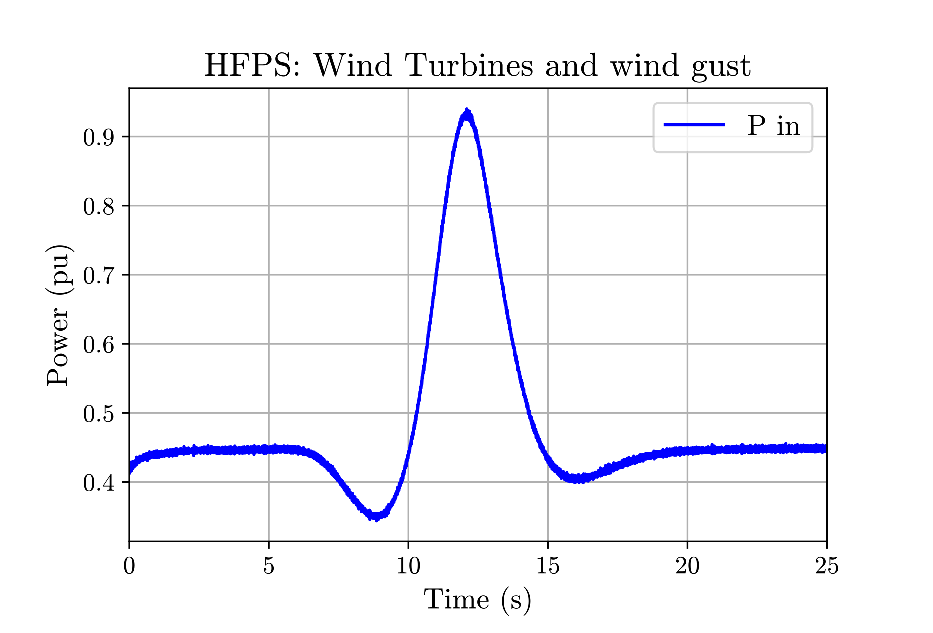
\includegraphics[scale=0.55]{figures/HFPS.eps}
        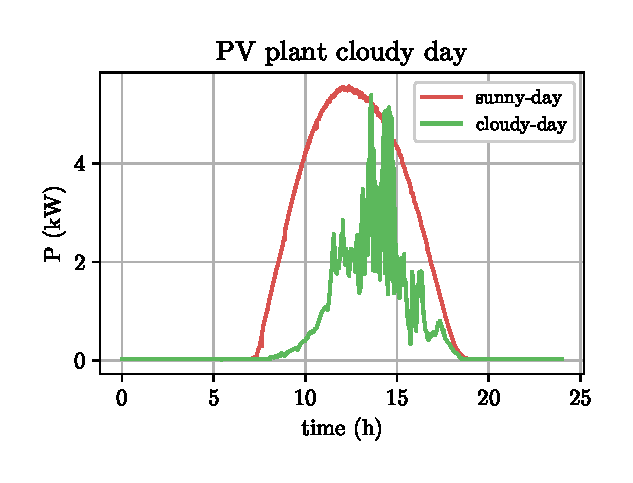
\includegraphics[scale=0.55]{figures/pv_cloudy-sunny.eps}
    \end{figure}
    
\end{frame}
%
%
\begin{frame}{¿Qué es el Power Smoothing?}
\begin{itemize}
    \item Acentuación de los problemas en redes débiles\\[1ex]
    \begin{itemize}
        \item Sistemas aislados, micro-redes \\[1ex]
        \item Grid Codes:
        \begin{itemize}
            \item PREPA (Puerto Rico): $10\% Pn/min$
            \item EirGrid (Irlanda): $30 MW/min$
            \item HECO (Hawai): $\pm2 MW/min$
            \item Denmark: $100 kW/s$ \\[1ex]
        \end{itemize}
        \item Tendencia a la penetración masiva de renovables \\[1ex]
        \item Tendencia a redes descentralizadas y autoconsumo \\[2ex]
    \end{itemize}{}
    \item Solución: Sistemas de almacenamiento energético (ESS)
    \begin{itemize}
        \item Super-condensadores  (SC)\\[1ex]
        \item Baterías (BESS)\\[1ex]
    \end{itemize}
    % Aquí habría que colocar aquí el esquema hardware
\end{itemize}
\end{frame}
%
%

